\section{Results}
\label{sec:res}

This section is structured as folows: First, Section~\ref{sec:seg4} demonstrates the level of segregation that can occur given our limited capability model with 4 neurons; Section~\ref{sec:seg6} demonstrates the behavior of a 6 neuron model; finally, Section~\ref{sec:fitness} discusses the performance our fitness search model. 


\subsection{Segregation with 4-neuron capability model}
\label{sec:seg4}

Our key contribution is to determine whether we can observe segregation with our given capability model. 
To determine this, we the previously described novelty search algorithm for 100 generations.
During each generation, we tested \emph{all permutations} of the 4 neuron weights with a step size of 0.1, which ensures that each step discover the true `most novel' new population.

At the end of this process, the population which demonstrated the highest segregation score had the weights $[0.61, 0.59, 0.01, 0.3]$. 
This can be interpreted as follows: when bot \emph{A} sees bot \emph{B} of the same type, it uses the first weights 0.61 and 0.59 to control its wheels.
This results in bot \emph{A} quickly moving generally straight (with a slight turn) towards the bot \emph{B}. 
When bot \emph{A} sees eithe nothing \emph{or} a bot of any other type, then the bot will use the second set of weights, 0.1, 0.3, to control its left and right wheels respectivly. 
This results in the bot mostly spinning in place until it sees a bot of the same type. 

This behavior can be seen in Figure~\ref{fig:init_pos_1} which depicts the positions of the bots over the course of the simulation. 
The colored depict the location of the bots at the start of the simulation and the light colored paths depict the locations of where the bots will travel. 
As seen here, the bots are evenly dispered at the start of the simulation, and thus not segregated.
The circling behavior can be seen at locations $X= 0$, $Y= -1.5$. 
The paths of the bots are drawn with low opacity, so the dark circle here demonstrates that a bot spent a great deal of time circling this location. 


\begin{figure}
    \centering
    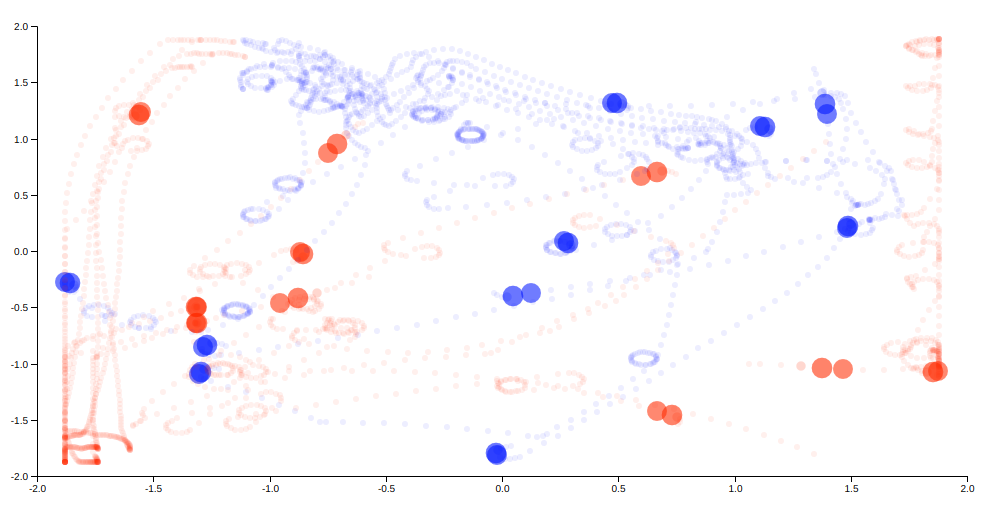
\includegraphics[width=\linewidth]{imgs/init_place_1.png}
    \caption{Positions of bots at the start of the simulation}
    \label{fig:init_pos_1}
\end{figure}

Figure~\ref{fig:final_seg_1} depicts our calculated segregation score for this population during each iteration. 
The highest segregation can be seen around step 2,400. 
The three values used to calulate this metric over the same time period are shown in Figure~\ref{fig:final_dev_1}. 
The line represent the standard deviation of the distances from the bots to the metroid of the cluster for each swarm with red line corresponding to the red group, the blue corresponding to the blue group, and the gray line corresponding to the total standard deviation of distances to the center of all bots. 
The dark colored dot depcits the current time in our animation~\footnote{We use a an interactive animation to depict these results. github:

\url{http://tiny.cc/e4hv5y}}.
Figure~\ref{fig:final_pos_1} demonstates the location of the bots during this point of highest segregation. 
As expected, when the bots look visually segregated, the intra-group standard deviations of their positions are low and the inter-group deviations are high (Figure~\ref{fig:final_dev_1}), and this corresponds to a high numeric value of segregation (Figure~\ref{fig:final_seg_1}). 

\begin{figure}
    \centering
    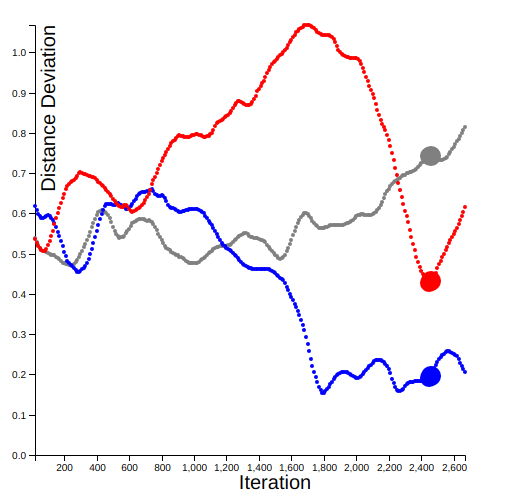
\includegraphics[width=5.5cm]{imgs/final_dev_1.png}
    \caption{Standard deviations of inter and intra-group distances for each population}
    \label{fig:final_dev_1}
\end{figure}

\begin{figure}
    \centering
    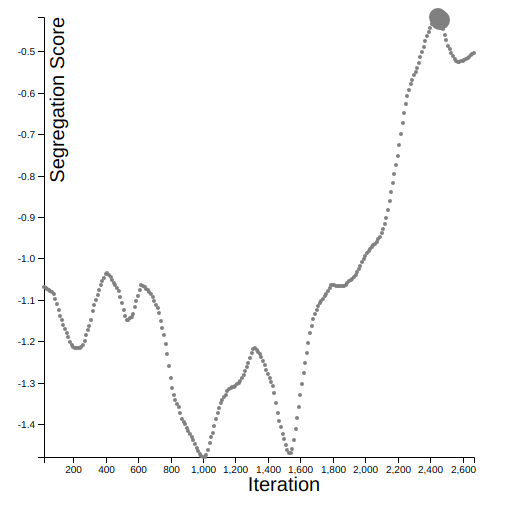
\includegraphics[width=5.5cm]{imgs/final_seg_1.png}
    \caption{Segregation score of the population at each time step}
    \label{fig:final_seg_1}
\end{figure}

\begin{figure}
    \centering
    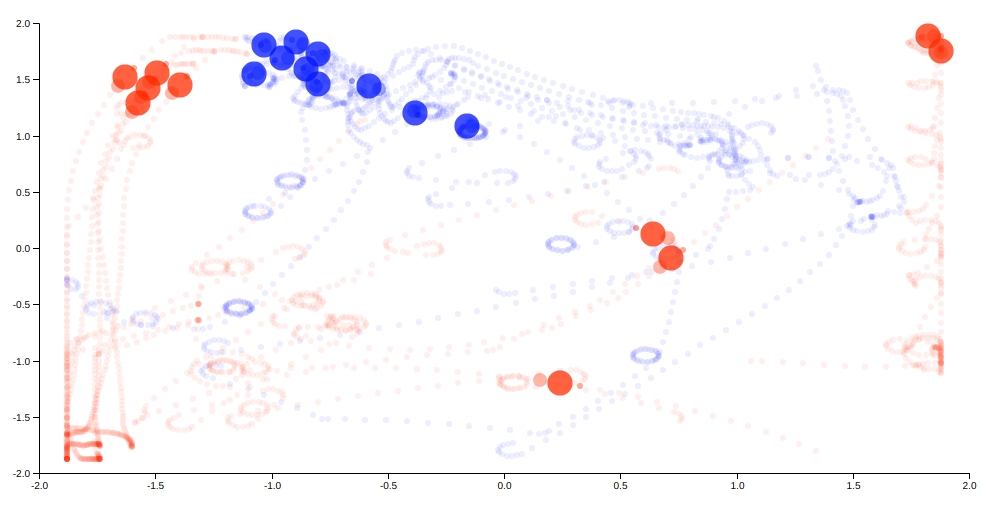
\includegraphics[width=\linewidth]{imgs/final_place_1.png}
    \caption{Positions of bots at the location of the highest clustering}
    \label{fig:final_pos_1}
\end{figure}

\subsection{Segregation with 6-neuron capability model}
\label{sec:seg6}


\subsection{Fitness search performance}
\label{sec:fitness}

NOTE: clean2 results are the fitness search results for 4 weights
